\clearpage
\part*{Part XI. The Higgs, Its Hub Register And The Dressing Field\\[5pt]{\large The (4,4) cell}}
\label{atlaspart:11-cell-4-4-higgs}
\addcontentsline{toc}{part}{Part XI. The Higgs, Its Hub Register And The Dressing Field, The (4,4) cell}
This Part reads the (4,4) cell. The expectation register of the hub, the vacuum register and the horizon cut register one register by construction, is to be read as a count of the Higgs sector at a later result, and that reading is stated here as an expectation and not as a claim of this Part.
\section{The Higgs: the closed hub read, its rows, its mass and its exponent}\label{mod:VI-10-higgs-the-closed-hub-read-its-rows-its-mass-and-its-exponent}
\chdesig{11-1}{6-10}{VI-10-higgs-the-closed-hub-read-its-rows-its-mass-and-its-exponent}{VI-10-D540200-hqrt-t1}
\label{narr:open:6-10}Theorem~200.1 reads the Higgs as the closed hub read, Theorem~200.2 its port, rows and weight, Theorem~200.3 its mass, vacuum port and exponent, and Open result~200.4 the three readings of the attachment; Open result~200.5 states the attachment at the saturated web as an open result and Theorem~200.6, a theorem, gives the Higgs and carrier offices at their sinks, the cells the register matrix prints.
\begin{chconditional}[The Higgs as the closed hub read]\label{box:VI-10-higgs-the-closed-hub-read-its-rows-its-mass-and-its-exponent:1}
Under the link lemmas, the body read at the lepton and the carriers from the readable genres, the Higgs word of the roster, the (4,4) attachment at ends of one dimension, is the closed read of its hub at the adopted closure, matched at the mass face and met again at the unit and the attachment: a carrier has a mass face if and only if it is closed at the ends of its chain, at all five catalogued carriers.
\end{chconditional}
\chstanding{conditional theorem}
\chdeps{the theorems of Chapters 1-0, 1-2 to 1-4, 1-6, 5-2 to 5-3, 8-3, 10-1}{the theorems of Chapters 1-1 to 1-2, 3-1, 5-3, 5-8f, 5-13, 6-3, 11-1}
The box reads the Higgs word, one link joining two ququarts, as the read whose hub is closed at both ends, and shows that the closure at the ends of a carrier chain is exactly what the prior link lemmas called a mass face, at every one of the five carriers.
\begin{chconditional}[The port, the rows and the weight of the Higgs word]\label{box:VI-10-higgs-the-closed-hub-read-its-rows-its-mass-and-its-exponent:2}
Under their parents, the port of the Higgs word is sealed at every clause, the one (4,4) link of the word unread at every clause; its four rows are keyed at every one of the seven distinct (3,4) junction legs of the six catalogued links, the unit the far end with the first power 12; and the Yukawa weight is the first power under its hub-pair name and no new object.
\end{chconditional}
\chstanding{conditional theorems, three}
\chdeps{the theorems of Chapters 1-0, 1-2 to 1-4, 1-6, 5-2 to 5-3, 8-3, 10-1}{the theorems of Chapters 1-1 to 1-2, 3-1, 5-3, 5-8f, 5-13, 6-3, 11-1}
The second box gathers three results on the same word, its link is never read, its rows live on the junction legs that join a qutrit to a ququart, and the weight the literature would call a Yukawa coupling is the first power already defined.
\begin{chconditional}[The mass, the vacuum port and the exponent]\label{box:VI-10-higgs-the-closed-hub-read-its-rows-its-mass-and-its-exponent:3}
Under their parents, the two faces of the Higgs mass are defined as exact objects at both port faces at the order-two attachment read; the primary port at the W word is the dock, the one port reading that is an output of the definition of open at the office, its register 6561 at the dock unit 67; and the direct two-exchange sum of the Higgs word equals the first power of its closed read and not its square, so the exponent is one and the word reads at the order two and no lower.
\end{chconditional}
\chstanding{conditional theorems, three}
\chdeps{the theorems of Chapters 1-0, 1-2 to 1-4, 1-6, 5-2 to 5-3, 8-3, 10-1}{the theorems of Chapters 1-1 to 1-2, 3-1, 5-3, 5-8f, 5-13, 6-3, 11-1}
The third box gives the mass as an exact object at two faces, names the port the vacuum register is read at, and fixes the exponent of the closed read at one.
\begin{chwall}[The three readings of the attachment]\label{box:VI-10-higgs-the-closed-hub-read-its-rows-its-mass-and-its-exponent:4}
The attachment is closed at the primary pair reading with the Higgs rows keyed at none of the four; the vacuum row parts the office rule at the leg unit; and the content cell of the attachment web is the singlet against the two-factor doublet, each an open result at its named step.
\end{chwall}
\chstanding{open results, three, built and not closed}
\chdeps{the theorems of Chapters 1-0, 1-2 to 1-4, 1-6, 5-2 to 5-3, 8-3, 10-1}{the theorems of Chapters 1-1 to 1-2, 3-1, 5-3, 5-8f, 5-13, 6-3, 11-1}
The fourth box names the three readings of the attachment that are tried and parted.
\begin{chbridge}
What this chapter calls the Higgs word the literature calls the Higgs boson, its closed hub read the Higgs field at its vacuum, the first power under the hub-pair name a Yukawa coupling, the vacuum register the vacuum expectation value and the exponent the order of the self-coupling, each by name only. The correspondence is by name, and every mass figure stands at the comparison table.
\end{chbridge}
\begin{chproof}[census]
The premises are the link and its six genres of chapter 1-2, the reads and the Born count of chapter 1-3 and the moves of chapter 1-4, definitions, the read at a register of chapter 1-6, the gauge chapters 4-2 and 4-3, the doublets of chapter 6-3 and the mass unit of chapter 8-1. The chain from the axiom to this chapter is eight chapters long. The set counted is the set of cataloged carriers, five words in the catalog order, the photon word, the W word, the Z word, the gluon word and the Higgs word, generated from the catalog of 64 webs, 1334 sites, 1691 links and 233 hub lines, every link genre equal to its two site dimensions at 1691 of 1691 and every hub line re-met from the sites and links at 233 of 233. The property tested is the closure at the ends of the carrier chain, every carrier a path with two ends. By kind the ends read. The photon word open, its ends of dimensions 2 and 3. The W word closed, its ends of dimension 4 and 4. The Z word closed, 4 and 4. The gluon word closed, 3 and 3. The Higgs word closed, and a mass face at the link lemmas stands at exactly the closed carriers, 5 of 5 matching, the first differing carrier none. The smallest case is the Higgs word itself, one (4,4) link,
\begin{equation}
16 = 4 \cdot 4 ,
\end{equation}
its rank and first power, no dock, its two hubs at in one and out none, the chain of one link closed at both ends and its mass face present. The exact part. From the electron web, the rank 79 less the two (2,3) docks at 6 each, we obtain the hub unit
\begin{equation}
67 = 79 - 12, \qquad 201 = 67 \cdot 3 ,
\end{equation}
the register of the closed hub at the dock and at the hub, re-met at 6 of 6 cells and at the nine chain bodies. From the attachment forcing at the closed hubs of the three closed words, six hubs at the room 3, the fresh far end is admitted at every dimension of the alphabet on the common support and its new pair read at none, the existing far ends consistent at 6966 candidates and the fresh far end consistent at 108 of 108 with the only consistent attachment at 0 of 108.

For the second and third boxes the typings of the port are counted at the rows the results name, zero on the read side and ten on the sealed side, the port struck from the rank 16 leaving the cut chain sum zero. The rows are keyed at the seven distinct (3,4) junction legs with the unit the far end at the first power 12. The records of the Higgs port are enumerated at the two-exchange register and the direct sum compared with the first power of the closed read and with its square, equal to the first and not the second, so the exponent is one. The vacuum register at the dock port is the square of the clauses register,
\begin{equation}
6561 = 81^{2} ,
\end{equation}
at the dock unit 67.

\emph{Check.} At the other four readings of the closure, the hub lines, the ports, the unit token and the face token, the match with the mass face fails at the photon word or the W word, as the closure table prints. The engines of this chapter were rerun with their captures equal byte for byte at every piece, so no cell moved. Each result was reproduced by an independent route, two engines at every capture byte for byte, its counter-tests at their pinned letters and its controls the same at both routes.
The open face of the attachment, the office rule at the leg unit and the content cell of the attachment web stay open. The mass unit and the first power are the matter of Part X.
\chcert{5}
\end{chproof}
\label{chend:VI-10-higgs-the-closed-hub-read-its-rows-its-mass-and-its-exponent}
\subsection{The Higgs attachment at the saturated web}\label{mod:VI-10-D536188-w-hgau}
\begin{chwall}[The Higgs attachment at the saturated web]\label{box:VI-10-D536188-w-hgau:1}
The Higgs attachment stands at the catalogued saturated sinks as their (4,4) links with the register 16 and the two faces of the attachment, the hub face at 16 and the leg face at 12, met again at every sink; the self-coupling, the vacuum value and the Higgs mass are exact displays at both faces, and the sink fixes the leg face where a (3,4) leg stands at a hub of its attachment link and neither face where none stands. On the one face the register is defined at every one of the 14666 attachment links; on the other face the face fixed by the sink is exactly one at 2372 of the 10123 attachment-bearing sinks, neither at 5716 and mixed at 2035, the first parting a proton sink fixing neither, named with both cells.
\end{chwall}
\chstanding{open result, built and not closed}
\chdeps{Definitions 1.1 to 1.6 and Theorems 200.1 to 200.3 and Open result 200.4}{no theorem beyond it at this release}
The box carries the attachment of the section above to every stable web of the saturation that bears one, finds the register the same everywhere, computes the three displays at both faces, and finds that the web alone does not say which face is the right one at more than half of them.
\begin{chbridge}
What this chapter calls the attachment the literature calls the coupling of the Higgs field, its self-coupling the quartic coupling, its vacuum value the vacuum expectation value and the Higgs mass the mass of the boson, each the nearest object by the rule of the section above and by name at the figure. The correspondence is by name, and the three displays are compared at the comparison table.
\end{chbridge}
\begin{chproof}[census]
The premises are the Higgs chapter above and the framework. The chain from the axiom to this result is nine chapters long. The set counted is the set of cataloged saturated sinks, 16962 webs from four sources, 14 of the roster, 16946 of the proton saturation, one of the bound-respecting seed and one lepton, parsed and equal to the census at the sites, links and genres at 16962 of 16962. The property tested is whether the sink bears the attachment, a (4,4) link, and which face its structure fixes. By kind. 10123 sinks bear the attachment as 14666 links of the genre (4,4), the register defined at 14666 of 14666 and equal to the Higgs word at the register 16. The face fixed by the sink at the adopted reading is the leg face at 2372, the hub face at 0, neither at 5716 and mixed at 2035, the first parting in the order of the material a proton sink fixing neither. The smallest case is one attachment link with its two faces, the hub face through both factors at the first power 16 and the leg face through one factor to the qutrit at the first power 12, with the self-coupling the Born square of the attachment read over the register and the vacuum value the register over the dock-struck electron unit 67,
\begin{equation}
\frac{256}{16} = 16, \qquad \frac{144}{16} = 9, \qquad \frac{16}{67} ,
\end{equation}
at the product register of the construction, and 1, 9/16 and 256/67 at the whole register beside. The mass displays at the two faces 16 over 67 and 12 over 67.

From the two faces of the attachment unit, 16 through both factors and 12 through one factor to the qutrit, equal to the faces of the parent result, by the census of the face fixed at the three readings, we obtain at the adopted reading 0 and 2372, at the pair reading 0 and 894, and at the available reading 8439 and 0, so the face fixed by the structure the read passes through and not uniformly across the saturated web. The unit of the construction, the dock-struck electron unit $79 - 12 = 67$, is re-derived from the catalog and equals the Yukawa bodies table and the attachment-read result.

\emph{Check.} One control of this result, the count of the catalog's closing lines, read 3446 against 3382 at the pinned engines, the bare closer of each block counted as a line, and 3382 at the precheck route and at the second-release engines with every deciding cell equal. Its fallback was recorded and did not fire. The result was reproduced by an independent route, two engines at every capture byte for byte, its counter-tests at their pinned letters.
The face of the attachment is fixed by the structure of each sink and by the saturated web as a whole not.
\chcert{14666}
\end{chproof}
\label{chend:VI-10-D536188-w-hgau}
\subsection{The Higgs and carrier offices at their sinks}\label{mod:VI-10-D538733-hcos-t1}
\begin{chtheorem}[The Higgs and carrier offices at their sinks]\label{box:VI-10-D538733-hcos-t1:1}
Every Higgs and carrier office of the compendium is an exact structure by the body-alone rule at the roster words: the closed-genre objects and the free genres are read at their own sinks, every office is an exact cell at every reading the results admit, and every ratio among them is an exact rational or ring cell, at all 52 ratios; the Higgs faces close 2 of 2, the carriers 6 of 6, and no sink the rule does not close and no ratio with no second read is found.
\end{chtheorem}
\chstanding{theorem}
\chdeps{Definitions 1.1 to 1.6, Theorem 195.1 and Theorems 200.1 to 200.3 and Open result 200.4}{no theorem beyond it at this release}
The box applies one rule, the office of a body read at its own stable web, to the Higgs word at both its faces and to the four carrier reads, and forms every ratio among the offices. Every office and every ratio comes out as an exact number of the ring.
\begin{chbridge}
What this chapter calls the Higgs office the literature calls the squared Higgs mass in the unit of the construction, the carrier offices the squared boson masses, and the stiffness the quartic coupling, each the nearest object. The correspondence is by name.
\end{chbridge}
\begin{chproof}[exact]
The premises are the Higgs chapter above and the body-alone office rule of chapter 8-2, a theorem, the chain from the axiom nine chapters long. The set counted is the reads the rule admits at the roster words, the Higgs word at both faces, the W and Z words at their cataloged webs, their closed-genre reads and the two free genres at one link each, with the 52 ratios among them, and the property tested is whether the rule closes the office as an exact cell. The exact part. From the Higgs word at the hub face, the (4,4) attachment at the register 16, by the first power squared plus the closure at the one dark link under the (4,4) law, we obtain the office
\begin{equation}
16^{2} + \frac{1681}{182250000} = \frac{46656001681}{182250000} ,
\end{equation}
and at the leg face, the (3,4) piece through one factor to the qutrit at the first power 12, the office $144$ plus a root-three closure, $4299817692073/29859840000 + (5069/373248000)\sqrt{3}$. From the W word at its cataloged web, the first power 28 with two (2,4) legs dark under the slot rule, we obtain the office
\begin{equation}
28^{2} + \frac{10241}{3645000} + \frac{98}{50625}\sqrt{2} = \frac{2857690241}{3645000} + \frac{98}{50625}\sqrt{2} ,
\end{equation}
the Z word the same web and its office the same, their ratio 1. By kind the offices close at 2 of 2 Higgs faces and 6 of 6 carrier reads, and the ratios are exact at 52 of 52, every one with a second read. The smallest ratio is the stiffness, the Higgs office at the hub face over the vacuum register $6561 = 81^{2}$,
\begin{equation}
\frac{46656001681}{182250000 \cdot 6561} = \frac{46656001681}{1195742250000} .
\end{equation}
\end{chproof}
\begin{chproof}[census]
The register of the attachment equals the Higgs word at 14666 of 14666 links across 10123 sinks, the first powers re-met at the carrier-mass, vacuum, scale-body and weak-angle results, and the first parting is none at either face.

\emph{Check.} The stiffness at the acts exponent and at the hub-port register reads 46656001681 over 14762250000 and over 46656000000, the office register re-met the same, and the result was reproduced by an independent route, its four counter-tests and sixteen controls at their pinned letters.
\chcert{52}
\end{chproof}
\begin{figure}[H]\centering
\begin{tikzpicture}[x=0.52pt,y=-0.52pt,baseline]
\clip (0,0) rectangle (900,540);
\fill[white] (0,0) rectangle (900,540);
\node[anchor=base west,inner sep=0pt,text=black,font=\fontsize{6.76}{8.112}\selectfont\ttfamily] at (12,22) {atlas r-hig: r-hig};
\node[anchor=base west,inner sep=0pt,text=black,font=\fontsize{6.24}{7.488}\selectfont\ttfamily] at (12,42) {membership 22:0;23:0;24:0;33:0;34:0;44:1; cells (4,4); links 1; sites 2; measure 16; census at the census};
\node[anchor=base west,inner sep=0pt,text=black,font=\fontsize{5.72}{6.864}\selectfont\ttfamily] at (12,62) {recorded office offices:HH:measure struck/slot/in-leg-34/R1/weight:HH=46656001681/182250000\textbar{}0\textbar{}0\textbar{}0; standing census:instrument;offices:theorem;formula:open result;roster:roster word; board Higgs};
\draw[draw=black,line width=1.04pt] (100,130) .. controls (130,110) and (160,110) .. (190,130);
\node[anchor=base,inner sep=0pt,text=black,font=\fontsize{5.72}{6.864}\selectfont\ttfamily] at (145,111) {(4,4)};
\filldraw[fill={rgb,255:red,112;green,112;blue,112},draw=black,line width=0.52pt] (100,130) circle (14);
\node[anchor=base,inner sep=0pt,text=white,font=\fontsize{6.24}{7.488}\selectfont\ttfamily] at (100,135) {4};
\node[anchor=base,inner sep=0pt,text=black,font=\fontsize{5.72}{6.864}\selectfont\ttfamily] at (100,160) {s1};
\filldraw[fill={rgb,255:red,112;green,112;blue,112},draw=black,line width=0.52pt] (190,130) circle (14);
\node[anchor=base,inner sep=0pt,text=white,font=\fontsize{6.24}{7.488}\selectfont\ttfamily] at (190,135) {4};
\node[anchor=base,inner sep=0pt,text=black,font=\fontsize{5.72}{6.864}\selectfont\ttfamily] at (190,160) {s2};
\node[anchor=base west,inner sep=0pt,text=black,font=\fontsize{5.72}{6.864}\selectfont\ttfamily] at (12,510) {the sites labelled by register (2 the qubit, white; 3 the qutrit, grey; 4 the ququart, dark); the links labelled by cell (p,q); a long dash an open dark link of the neutron row; a short dash a docked link at the rule R1};
\end{tikzpicture}
\caption{\texttt{r-hig} (the Higgs), Higgs: 2 sites, 1 links, the measure 16; the links at the cells (4,4); the membership 22:0; 23:0; 24:0; 33:0; 34:0; 44:1; dock-free at the rule R1; at the census of the six cells. Drawn at the anatomy atlas as its web, the sites labeled by register and the links by cell, from the the Higgs and carrier offices at their sinks.}\label{fig:VI-10-D538733-r-hig-55890f}
\begin{center}\footnotesize\begin{adjustbox}{max width=\linewidth}\begin{tabular}{p{0.26\textwidth}p{0.68\textwidth}}\toprule
recorded office (the slot-count row) & the read o-hh of the formula row: the first power 16; the office \texttt{46656001681/182250000\textbar{}0\textbar{}0\textbar{}0}; against the formula with the slot count equal; the slot total 0; dark links 1; hubs none; dressing 1 \\
mass register (the mass-register row) & the read HH: the class touching the ququart; the first power 16; the office \texttt{46656001681/182250000\textbar{}0\textbar{}0\textbar{}0}; nonzero; met yes; hubs none; in-legs none; dressing 1; ports s1-s2 \\
\bottomrule\end{tabular}\end{adjustbox}\end{center}
\end{figure}
\begin{figure}[H]\centering
\begin{tikzpicture}[x=0.52pt,y=-0.52pt,baseline]
\clip (0,0) rectangle (900,540);
\fill[white] (0,0) rectangle (900,540);
\node[anchor=base west,inner sep=0pt,text=black,font=\fontsize{6.76}{8.112}\selectfont\ttfamily] at (12,22) {atlas offices:F34: free-genre-(3,4)};
\node[anchor=base west,inner sep=0pt,text=black,font=\fontsize{6.24}{7.488}\selectfont\ttfamily] at (12,42) {membership 22:0;23:0;24:0;33:0;34:1;44:0; cells (3,4); links 1; sites 2; measure 12; census at the census};
\node[anchor=base west,inner sep=0pt,text=black,font=\fontsize{5.72}{6.864}\selectfont\ttfamily] at (12,62) {recorded office offices:F34:measure struck/slot/in-leg-34/R1/weight:F34=4299817692073/29859840000\textbar{}0\textbar{}5069/373248000\textbar{}0; standing census:instrument;offices:theorem;formula:open result; board none};
\draw[draw=black,line width=1.04pt] (100,470) .. controls (130,450) and (160,450) .. (190,470);
\node[anchor=base,inner sep=0pt,text=black,font=\fontsize{5.72}{6.864}\selectfont\ttfamily] at (145,451) {(3,4)};
\filldraw[fill={rgb,255:red,244;green,192;blue,192},draw=black,line width=0.52pt] (100,470) circle (14);
\node[anchor=base,inner sep=0pt,text=black,font=\fontsize{6.24}{7.488}\selectfont\ttfamily] at (100,475) {0};
\node[anchor=base,inner sep=0pt,text=black,font=\fontsize{5.72}{6.864}\selectfont\ttfamily] at (100,500) {x3};
\filldraw[fill={rgb,255:red,244;green,192;blue,192},draw=black,line width=0.52pt] (190,470) circle (14);
\node[anchor=base,inner sep=0pt,text=black,font=\fontsize{6.24}{7.488}\selectfont\ttfamily] at (190,475) {0};
\node[anchor=base,inner sep=0pt,text=black,font=\fontsize{5.72}{6.864}\selectfont\ttfamily] at (190,500) {y4};
\node[anchor=base west,inner sep=0pt,text=black,font=\fontsize{5.72}{6.864}\selectfont\ttfamily] at (12,510) {the sites labelled by register (2 the qubit, white; 3 the qutrit, grey; 4 the ququart, dark); the links labelled by cell (p,q); a long dash an open dark link of the neutron row; a short dash a docked link at the rule R1};
\end{tikzpicture}
\caption{\texttt{free-genre-(3,4)}, free: 2 sites, 1 links, the measure 12; the links at the cells (3,4); the membership 22:0; 23:0; 24:0; 33:0; 34:1; 44:0; dock-free at the rule R1; at the census of the six cells; 2 sites at the fourth band with the register unresolved by the genre alone, the drawing gloss not drawn at them as the compendium prints it. Drawn at the anatomy atlas as its web, the sites labeled by register and the links by cell, from the the Higgs and carrier offices at their sinks.}\label{fig:VI-10-D538733-free-genre-3-4-131d45}
\begin{center}\footnotesize\begin{adjustbox}{max width=\linewidth}\begin{tabular}{p{0.26\textwidth}p{0.68\textwidth}}\toprule
recorded office (the slot-count row) & the read O-F34 of the formula row: the first power 12; the office \texttt{4299817692073/29859840000\textbar{}0\textbar{}5069/373248000\textbar{}0}; against the formula with the slot count equal; the slot total 0; dark links 1; hubs none; dressing 1 \\
mass register (the mass-register row) & the read F34: the class touching the ququart; the first power 12; the office \texttt{4299817692073/29859840000\textbar{}0\textbar{}5069/373248000\textbar{}0}; nonzero; met yes; hubs none; in-legs none; dressing 1; ports x3-y4 \\
\bottomrule\end{tabular}\end{adjustbox}\end{center}
\end{figure}
\begin{figure}[H]\centering
\begin{tikzpicture}[x=0.52pt,y=-0.52pt,baseline]
\clip (0,0) rectangle (900,540);
\fill[white] (0,0) rectangle (900,540);
\node[anchor=base west,inner sep=0pt,text=black,font=\fontsize{6.76}{8.112}\selectfont\ttfamily] at (12,22) {atlas offices:HL: leg-piece-(3,4)};
\node[anchor=base west,inner sep=0pt,text=black,font=\fontsize{6.24}{7.488}\selectfont\ttfamily] at (12,42) {membership 22:0;23:0;24:0;33:0;34:1;44:0; cells (3,4); links 1; sites 2; measure 12; census at the census};
\node[anchor=base west,inner sep=0pt,text=black,font=\fontsize{5.72}{6.864}\selectfont\ttfamily] at (12,62) {recorded office offices:HL:measure struck/slot/in-leg-34/R1/weight:HL=4299817692073/29859840000\textbar{}0\textbar{}5069/373248000\textbar{}0; standing census:instrument;offices:theorem;formula:open result; board none};
\draw[draw=black,line width=1.04pt] (100,470) .. controls (130,450) and (160,450) .. (190,470);
\node[anchor=base,inner sep=0pt,text=black,font=\fontsize{5.72}{6.864}\selectfont\ttfamily] at (145,451) {(3,4)};
\filldraw[fill={rgb,255:red,244;green,192;blue,192},draw=black,line width=0.52pt] (100,470) circle (14);
\node[anchor=base,inner sep=0pt,text=black,font=\fontsize{6.24}{7.488}\selectfont\ttfamily] at (100,475) {0};
\node[anchor=base,inner sep=0pt,text=black,font=\fontsize{5.72}{6.864}\selectfont\ttfamily] at (100,500) {h};
\filldraw[fill={rgb,255:red,244;green,192;blue,192},draw=black,line width=0.52pt] (190,470) circle (14);
\node[anchor=base,inner sep=0pt,text=black,font=\fontsize{6.24}{7.488}\selectfont\ttfamily] at (190,475) {0};
\node[anchor=base,inner sep=0pt,text=black,font=\fontsize{5.72}{6.864}\selectfont\ttfamily] at (190,500) {q};
\node[anchor=base west,inner sep=0pt,text=black,font=\fontsize{5.72}{6.864}\selectfont\ttfamily] at (12,510) {the sites labelled by register (2 the qubit, white; 3 the qutrit, grey; 4 the ququart, dark); the links labelled by cell (p,q); a long dash an open dark link of the neutron row; a short dash a docked link at the rule R1};
\end{tikzpicture}
\caption{\texttt{leg-piece-(3,4)}, Higgs: 2 sites, 1 links, the measure 12; the links at the cells (3,4); the membership 22:0; 23:0; 24:0; 33:0; 34:1; 44:0; dock-free at the rule R1; at the census of the six cells; 2 sites at the fourth band with the register unresolved by the genre alone, the drawing gloss not drawn at them as the compendium prints it. Drawn at the anatomy atlas as its web, the sites labeled by register and the links by cell, from the the Higgs and carrier offices at their sinks.}\label{fig:VI-10-D538733-leg-piece-3-4-5a3770}
\begin{center}\footnotesize\begin{adjustbox}{max width=\linewidth}\begin{tabular}{p{0.26\textwidth}p{0.68\textwidth}}\toprule
recorded office (the slot-count row) & the read o-hl of the formula row: the first power 12; the office \texttt{4299817692073/29859840000\textbar{}0\textbar{}5069/373248000\textbar{}0}; against the formula with the slot count equal; the slot total 0; dark links 1; hubs none; dressing 1 \\
mass register (the mass-register row) & the read HL: the class touching the ququart; the first power 12; the office \texttt{4299817692073/29859840000\textbar{}0\textbar{}5069/373248000\textbar{}0}; nonzero; met yes; hubs none; in-legs none; dressing 1; ports h-q \\
\bottomrule\end{tabular}\end{adjustbox}\end{center}
\end{figure}
\begin{figure}[H]\centering
\begin{tikzpicture}[x=0.52pt,y=-0.52pt,baseline]
\clip (0,0) rectangle (900,540);
\fill[white] (0,0) rectangle (900,540);
\node[anchor=base west,inner sep=0pt,text=black,font=\fontsize{6.76}{8.112}\selectfont\ttfamily] at (12,22) {atlas offices:F24: free-genre-(2,4)};
\node[anchor=base west,inner sep=0pt,text=black,font=\fontsize{6.24}{7.488}\selectfont\ttfamily] at (12,42) {membership 22:0;23:0;24:1;33:0;34:0;44:0; cells (2,4); links 1; sites 2; measure 8; census at the census};
\node[anchor=base west,inner sep=0pt,text=black,font=\fontsize{5.72}{6.864}\selectfont\ttfamily] at (12,62) {recorded office offices:F24:measure struck/slot/in-leg-34/R1/weight:F24=466566137/7290000\textbar{}2/6075\textbar{}0\textbar{}0; standing census:instrument;offices:theorem;formula:open result; board none};
\draw[draw=black,line width=1.04pt] (100,470) .. controls (130,450) and (160,450) .. (190,470);
\node[anchor=base,inner sep=0pt,text=black,font=\fontsize{5.72}{6.864}\selectfont\ttfamily] at (145,451) {(2,4)};
\filldraw[fill={rgb,255:red,244;green,192;blue,192},draw=black,line width=0.52pt] (100,470) circle (14);
\node[anchor=base,inner sep=0pt,text=black,font=\fontsize{6.24}{7.488}\selectfont\ttfamily] at (100,475) {0};
\node[anchor=base,inner sep=0pt,text=black,font=\fontsize{5.72}{6.864}\selectfont\ttfamily] at (100,500) {x2};
\filldraw[fill={rgb,255:red,244;green,192;blue,192},draw=black,line width=0.52pt] (190,470) circle (14);
\node[anchor=base,inner sep=0pt,text=black,font=\fontsize{6.24}{7.488}\selectfont\ttfamily] at (190,475) {0};
\node[anchor=base,inner sep=0pt,text=black,font=\fontsize{5.72}{6.864}\selectfont\ttfamily] at (190,500) {y4};
\node[anchor=base west,inner sep=0pt,text=black,font=\fontsize{5.72}{6.864}\selectfont\ttfamily] at (12,510) {the sites labelled by register (2 the qubit, white; 3 the qutrit, grey; 4 the ququart, dark); the links labelled by cell (p,q); a long dash an open dark link of the neutron row; a short dash a docked link at the rule R1};
\end{tikzpicture}
\caption{\texttt{free-genre-(2,4)}, free: 2 sites, 1 links, the measure 8; the links at the cells (2,4); the membership 22:0; 23:0; 24:1; 33:0; 34:0; 44:0; dock-free at the rule R1; at the census of the six cells; 2 sites at the fourth band with the register unresolved by the genre alone, the drawing gloss not drawn at them as the compendium prints it. Drawn at the anatomy atlas as its web, the sites labeled by register and the links by cell, from the the Higgs and carrier offices at their sinks.}\label{fig:VI-10-D538733-free-genre-2-4-e1956c}
\begin{center}\footnotesize\begin{adjustbox}{max width=\linewidth}\begin{tabular}{p{0.26\textwidth}p{0.68\textwidth}}\toprule
recorded office (the slot-count row) & the read O-F24 of the formula row: the first power 8; the office \texttt{466566137/7290000\textbar{}2/6075\textbar{}0\textbar{}0}; against the formula with the slot count equal; the slot total 0; dark links 1; hubs none; dressing 1 \\
mass register (the mass-register row) & the read F24: the class touching the ququart; the first power 8; the office \texttt{466566137/7290000\textbar{}2/6075\textbar{}0\textbar{}0}; nonzero; met yes; hubs none; in-legs none; dressing 1; ports x2-y4 \\
\bottomrule\end{tabular}\end{adjustbox}\end{center}
\end{figure}
\begin{figure}[H]\centering
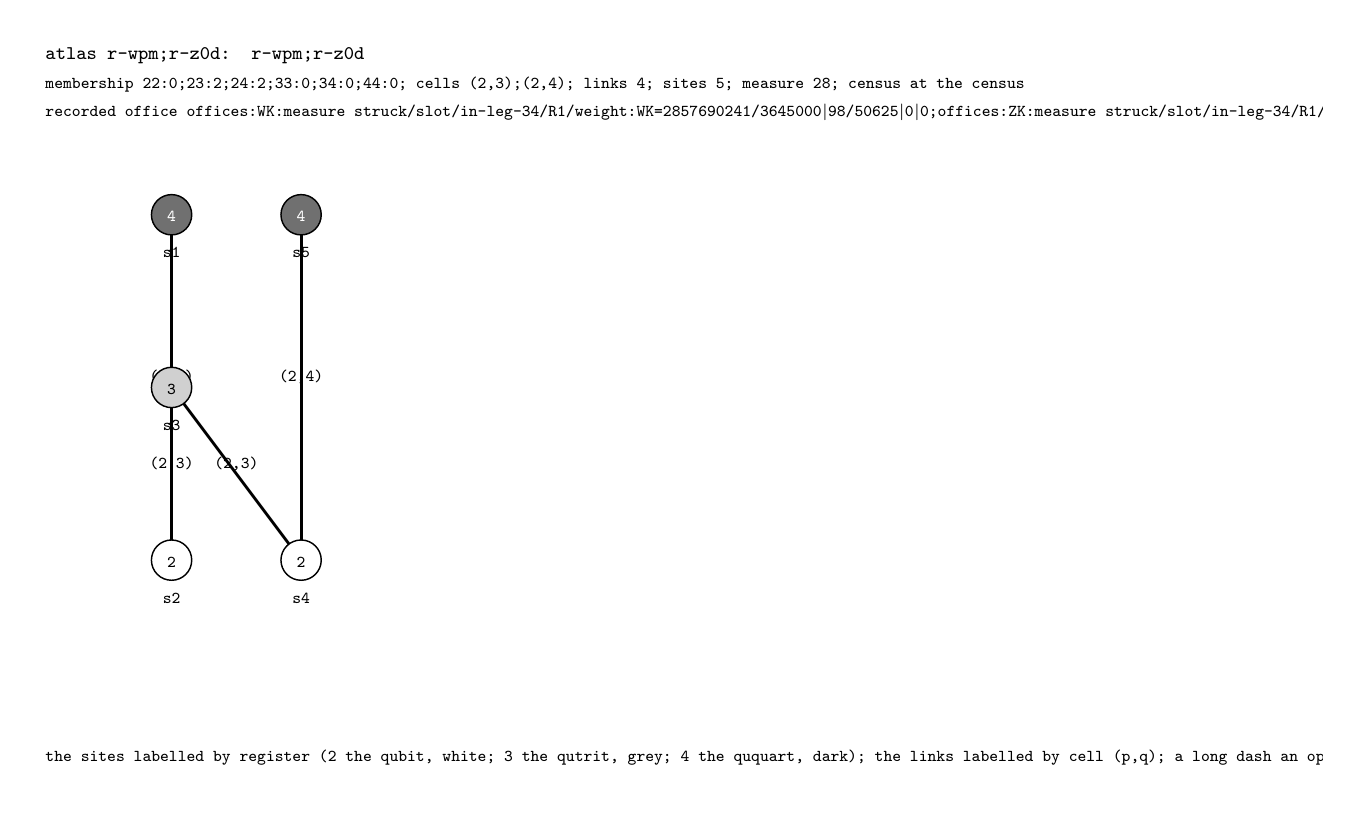
\begin{tikzpicture}[x=0.52pt,y=-0.52pt,baseline]
\clip (0,0) rectangle (900,540);
\fill[white] (0,0) rectangle (900,540);
\node[anchor=base west,inner sep=0pt,text=black,font=\fontsize{6.76}{8.112}\selectfont\ttfamily] at (12,22) {atlas r-wpm;r-z0d: r-wpm;r-z0d};
\node[anchor=base west,inner sep=0pt,text=black,font=\fontsize{6.24}{7.488}\selectfont\ttfamily] at (12,42) {membership 22:0;23:2;24:2;33:0;34:0;44:0; cells (2,3);(2,4); links 4; sites 5; measure 28; census at the census};
\node[anchor=base west,inner sep=0pt,text=black,font=\fontsize{5.72}{6.864}\selectfont\ttfamily] at (12,62) {recorded office offices:WK:measure struck/slot/in-leg-34/R1/weight:WK=2857690241/3645000\textbar{}98/50625\textbar{}0\textbar{}0;offices:ZK:measure struck/slot/in-leg-34/R1/weight:ZK=2857690241/3645000\textbar{}98/50625\textbar{}0\textbar{}0; standing census:instrument;offices:theorem;formula:open result;roster:roster word; board W};
\draw[draw=black,line width=1.04pt] (100,130) -- (100,370);
\node[anchor=base,inner sep=0pt,text=black,font=\fontsize{5.72}{6.864}\selectfont\ttfamily] at (100,246) {(2,4)};
\draw[draw=black,line width=1.04pt] (100,370) -- (100,250);
\node[anchor=base,inner sep=0pt,text=black,font=\fontsize{5.72}{6.864}\selectfont\ttfamily] at (100,306) {(2,3)};
\draw[draw=black,line width=1.04pt] (100,250) -- (190,370);
\node[anchor=base,inner sep=0pt,text=black,font=\fontsize{5.72}{6.864}\selectfont\ttfamily] at (145,306) {(2,3)};
\draw[draw=black,line width=1.04pt] (190,370) -- (190,130);
\node[anchor=base,inner sep=0pt,text=black,font=\fontsize{5.72}{6.864}\selectfont\ttfamily] at (190,246) {(2,4)};
\filldraw[fill={rgb,255:red,112;green,112;blue,112},draw=black,line width=0.52pt] (100,130) circle (14);
\node[anchor=base,inner sep=0pt,text=white,font=\fontsize{6.24}{7.488}\selectfont\ttfamily] at (100,135) {4};
\node[anchor=base,inner sep=0pt,text=black,font=\fontsize{5.72}{6.864}\selectfont\ttfamily] at (100,160) {s1};
\filldraw[fill=white,draw=black,line width=0.52pt] (100,370) circle (14);
\node[anchor=base,inner sep=0pt,text=black,font=\fontsize{6.24}{7.488}\selectfont\ttfamily] at (100,375) {2};
\node[anchor=base,inner sep=0pt,text=black,font=\fontsize{5.72}{6.864}\selectfont\ttfamily] at (100,400) {s2};
\filldraw[fill={rgb,255:red,208;green,208;blue,208},draw=black,line width=0.52pt] (100,250) circle (14);
\node[anchor=base,inner sep=0pt,text=black,font=\fontsize{6.24}{7.488}\selectfont\ttfamily] at (100,255) {3};
\node[anchor=base,inner sep=0pt,text=black,font=\fontsize{5.72}{6.864}\selectfont\ttfamily] at (100,280) {s3};
\filldraw[fill=white,draw=black,line width=0.52pt] (190,370) circle (14);
\node[anchor=base,inner sep=0pt,text=black,font=\fontsize{6.24}{7.488}\selectfont\ttfamily] at (190,375) {2};
\node[anchor=base,inner sep=0pt,text=black,font=\fontsize{5.72}{6.864}\selectfont\ttfamily] at (190,400) {s4};
\filldraw[fill={rgb,255:red,112;green,112;blue,112},draw=black,line width=0.52pt] (190,130) circle (14);
\node[anchor=base,inner sep=0pt,text=white,font=\fontsize{6.24}{7.488}\selectfont\ttfamily] at (190,135) {4};
\node[anchor=base,inner sep=0pt,text=black,font=\fontsize{5.72}{6.864}\selectfont\ttfamily] at (190,160) {s5};
\node[anchor=base west,inner sep=0pt,text=black,font=\fontsize{5.72}{6.864}\selectfont\ttfamily] at (12,510) {the sites labelled by register (2 the qubit, white; 3 the qutrit, grey; 4 the ququart, dark); the links labelled by cell (p,q); a long dash an open dark link of the neutron row; a short dash a docked link at the rule R1};
\end{tikzpicture}
\caption{\texttt{r-wpm; r-z0d} (the W word), carrier: 5 sites, 4 links, the measure 28; the links at the cells (2,3), (2,4); the membership 22:0; 23:2; 24:2; 33:0; 34:0; 44:0; dock-free at the rule R1; at the census of the six cells. Drawn at the anatomy atlas as its web, the sites labeled by register and the links by cell, from the the Higgs and carrier offices at their sinks.}\label{fig:VI-10-D538733-r-wpm-d8dad0}
\begin{center}\footnotesize\begin{adjustbox}{max width=\linewidth}\begin{tabular}{p{0.26\textwidth}p{0.68\textwidth}}\toprule
recorded office (the slot-count row) & the read o-wk of the formula row: the first power 28; the office \texttt{2857690241/3645000\textbar{}98/50625\textbar{}0\textbar{}0}; against the formula with the slot count equal; the slot total 2; dark links 2; hubs none; dressing 1 \\
mass register (the mass-register row) & the read WK: the class touching the ququart; the first power 28; the office \texttt{2857690241/3645000\textbar{}98/50625\textbar{}0\textbar{}0}; nonzero; met yes; hubs none; in-legs none; dressing 1; ports s1-s2; s4-s5 \\
\bottomrule\end{tabular}\end{adjustbox}\end{center}
\end{figure}
\begin{figure}[H]\centering
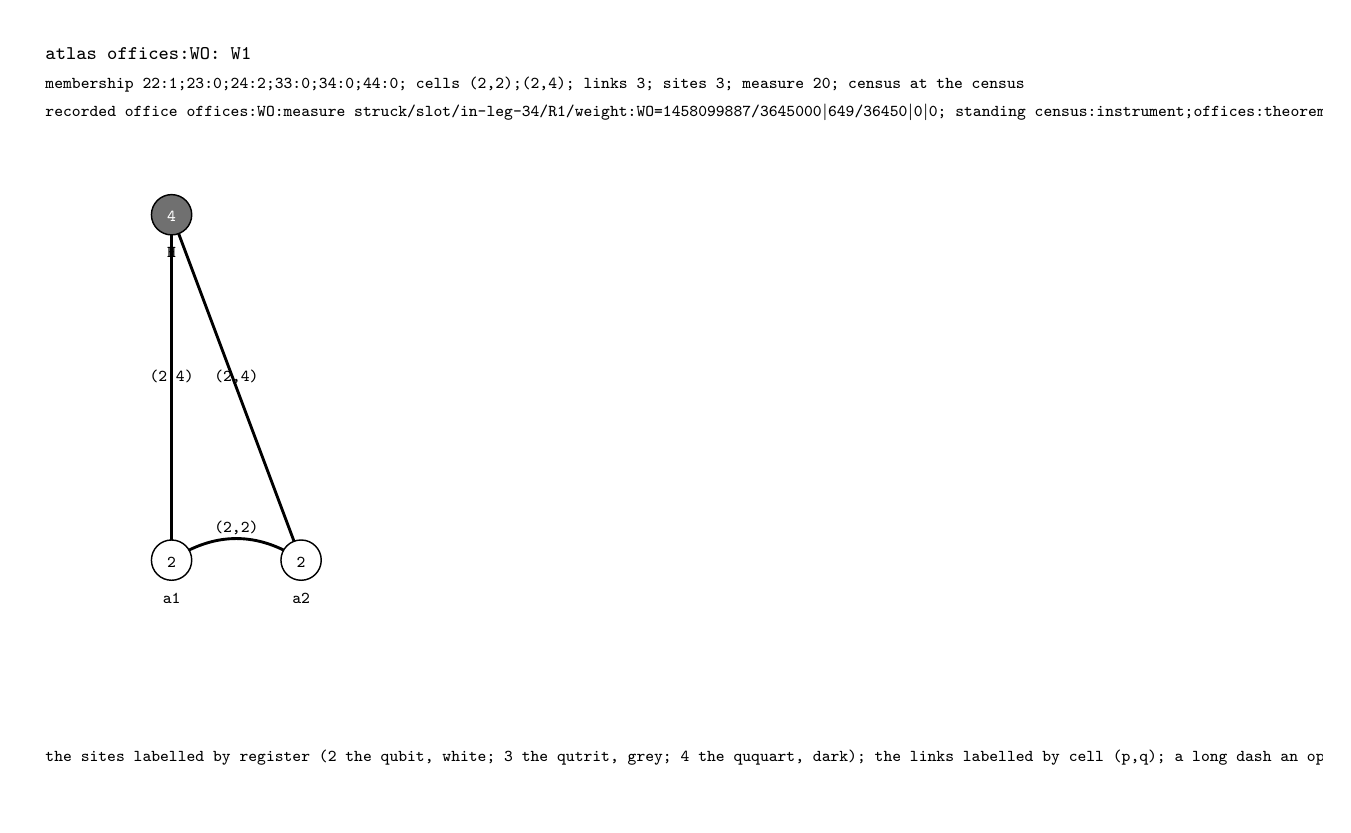
\begin{tikzpicture}[x=0.52pt,y=-0.52pt,baseline]
\clip (0,0) rectangle (900,540);
\fill[white] (0,0) rectangle (900,540);
\node[anchor=base west,inner sep=0pt,text=black,font=\fontsize{6.76}{8.112}\selectfont\ttfamily] at (12,22) {atlas offices:WO: W1};
\node[anchor=base west,inner sep=0pt,text=black,font=\fontsize{6.24}{7.488}\selectfont\ttfamily] at (12,42) {membership 22:1;23:0;24:2;33:0;34:0;44:0; cells (2,2);(2,4); links 3; sites 3; measure 20; census at the census};
\node[anchor=base west,inner sep=0pt,text=black,font=\fontsize{5.72}{6.864}\selectfont\ttfamily] at (12,62) {recorded office offices:WO:measure struck/slot/in-leg-34/R1/weight:WO=1458099887/3645000\textbar{}649/36450\textbar{}0\textbar{}0; standing census:instrument;offices:theorem;formula:open result; board none};
\draw[draw=black,line width=1.04pt] (100,130) -- (100,370);
\node[anchor=base,inner sep=0pt,text=black,font=\fontsize{5.72}{6.864}\selectfont\ttfamily] at (100,246) {(2,4)};
\draw[draw=black,line width=1.04pt] (100,130) -- (190,370);
\node[anchor=base,inner sep=0pt,text=black,font=\fontsize{5.72}{6.864}\selectfont\ttfamily] at (145,246) {(2,4)};
\draw[draw=black,line width=1.04pt] (100,370) .. controls (130,350) and (160,350) .. (190,370);
\node[anchor=base,inner sep=0pt,text=black,font=\fontsize{5.72}{6.864}\selectfont\ttfamily] at (145,351) {(2,2)};
\filldraw[fill={rgb,255:red,112;green,112;blue,112},draw=black,line width=0.52pt] (100,130) circle (14);
\node[anchor=base,inner sep=0pt,text=white,font=\fontsize{6.24}{7.488}\selectfont\ttfamily] at (100,135) {4};
\node[anchor=base,inner sep=0pt,text=black,font=\fontsize{5.72}{6.864}\selectfont\ttfamily] at (100,160) {H};
\filldraw[fill=white,draw=black,line width=0.52pt] (100,370) circle (14);
\node[anchor=base,inner sep=0pt,text=black,font=\fontsize{6.24}{7.488}\selectfont\ttfamily] at (100,375) {2};
\node[anchor=base,inner sep=0pt,text=black,font=\fontsize{5.72}{6.864}\selectfont\ttfamily] at (100,400) {a1};
\filldraw[fill=white,draw=black,line width=0.52pt] (190,370) circle (14);
\node[anchor=base,inner sep=0pt,text=black,font=\fontsize{6.24}{7.488}\selectfont\ttfamily] at (190,375) {2};
\node[anchor=base,inner sep=0pt,text=black,font=\fontsize{5.72}{6.864}\selectfont\ttfamily] at (190,400) {a2};
\node[anchor=base west,inner sep=0pt,text=black,font=\fontsize{5.72}{6.864}\selectfont\ttfamily] at (12,510) {the sites labelled by register (2 the qubit, white; 3 the qutrit, grey; 4 the ququart, dark); the links labelled by cell (p,q); a long dash an open dark link of the neutron row; a short dash a docked link at the rule R1};
\end{tikzpicture}
\caption{\texttt{W1}, carrier: 3 sites, 3 links, the measure 20; the links at the cells (2,2), (2,4); the membership 22:1; 23:0; 24:2; 33:0; 34:0; 44:0; dock-free at the rule R1; at the census of the six cells. Drawn at the anatomy atlas as its web, the sites labeled by register and the links by cell, from the the Higgs and carrier offices at their sinks.}\label{fig:VI-10-D538733-w1-e857e4}
\begin{center}\footnotesize\begin{adjustbox}{max width=\linewidth}\begin{tabular}{p{0.26\textwidth}p{0.68\textwidth}}\toprule
recorded office (the slot-count row) & the read o-wo of the formula row: the first power 20; the office \texttt{1458099887/3645000\textbar{}649/36450\textbar{}0\textbar{}0}; against the formula with the slot count equal; the slot total 0; dark links 3; hubs none; dressing 1 \\
mass register (the mass-register row) & the read WO: the class touching the ququart; the first power 20; the office \texttt{1458099887/3645000\textbar{}649/36450\textbar{}0\textbar{}0}; nonzero; met yes; hubs none; in-legs none; dressing 1; ports none \\
\bottomrule\end{tabular}\end{adjustbox}\end{center}
\end{figure}
\begin{figure}[H]\centering
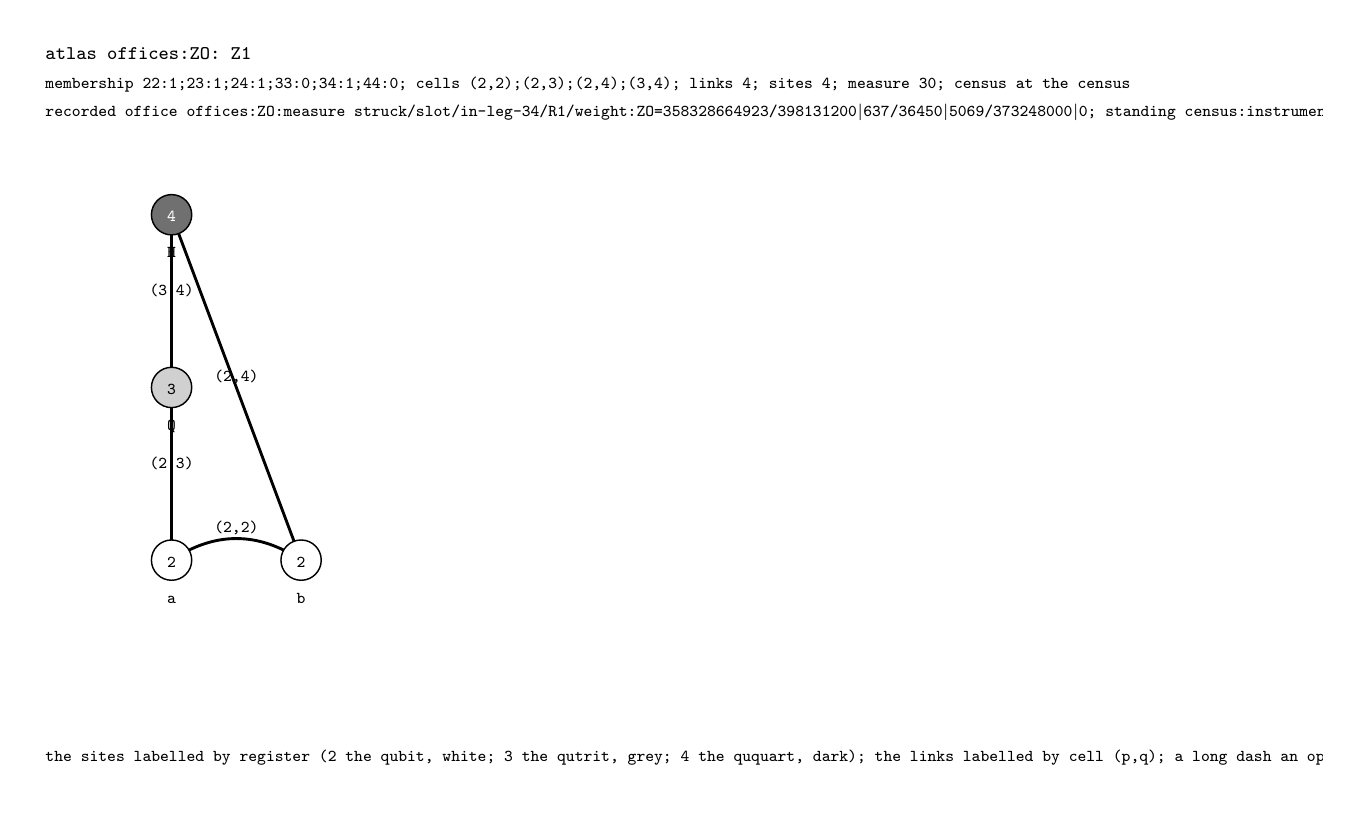
\begin{tikzpicture}[x=0.52pt,y=-0.52pt,baseline]
\clip (0,0) rectangle (900,540);
\fill[white] (0,0) rectangle (900,540);
\node[anchor=base west,inner sep=0pt,text=black,font=\fontsize{6.76}{8.112}\selectfont\ttfamily] at (12,22) {atlas offices:ZO: Z1};
\node[anchor=base west,inner sep=0pt,text=black,font=\fontsize{6.24}{7.488}\selectfont\ttfamily] at (12,42) {membership 22:1;23:1;24:1;33:0;34:1;44:0; cells (2,2);(2,3);(2,4);(3,4); links 4; sites 4; measure 30; census at the census};
\node[anchor=base west,inner sep=0pt,text=black,font=\fontsize{5.72}{6.864}\selectfont\ttfamily] at (12,62) {recorded office offices:ZO:measure struck/slot/in-leg-34/R1/weight:ZO=358328664923/398131200\textbar{}637/36450\textbar{}5069/373248000\textbar{}0; standing census:instrument;offices:theorem;formula:open result; board none};
\draw[draw=black,line width=1.04pt] (100,130) -- (100,250);
\node[anchor=base,inner sep=0pt,text=black,font=\fontsize{5.72}{6.864}\selectfont\ttfamily] at (100,186) {(3,4)};
\draw[draw=black,line width=1.04pt] (100,130) -- (190,370);
\node[anchor=base,inner sep=0pt,text=black,font=\fontsize{5.72}{6.864}\selectfont\ttfamily] at (145,246) {(2,4)};
\draw[draw=black,line width=1.04pt] (100,250) -- (100,370);
\node[anchor=base,inner sep=0pt,text=black,font=\fontsize{5.72}{6.864}\selectfont\ttfamily] at (100,306) {(2,3)};
\draw[draw=black,line width=1.04pt] (100,370) .. controls (130,350) and (160,350) .. (190,370);
\node[anchor=base,inner sep=0pt,text=black,font=\fontsize{5.72}{6.864}\selectfont\ttfamily] at (145,351) {(2,2)};
\filldraw[fill={rgb,255:red,112;green,112;blue,112},draw=black,line width=0.52pt] (100,130) circle (14);
\node[anchor=base,inner sep=0pt,text=white,font=\fontsize{6.24}{7.488}\selectfont\ttfamily] at (100,135) {4};
\node[anchor=base,inner sep=0pt,text=black,font=\fontsize{5.72}{6.864}\selectfont\ttfamily] at (100,160) {H};
\filldraw[fill={rgb,255:red,208;green,208;blue,208},draw=black,line width=0.52pt] (100,250) circle (14);
\node[anchor=base,inner sep=0pt,text=black,font=\fontsize{6.24}{7.488}\selectfont\ttfamily] at (100,255) {3};
\node[anchor=base,inner sep=0pt,text=black,font=\fontsize{5.72}{6.864}\selectfont\ttfamily] at (100,280) {Q};
\filldraw[fill=white,draw=black,line width=0.52pt] (100,370) circle (14);
\node[anchor=base,inner sep=0pt,text=black,font=\fontsize{6.24}{7.488}\selectfont\ttfamily] at (100,375) {2};
\node[anchor=base,inner sep=0pt,text=black,font=\fontsize{5.72}{6.864}\selectfont\ttfamily] at (100,400) {a};
\filldraw[fill=white,draw=black,line width=0.52pt] (190,370) circle (14);
\node[anchor=base,inner sep=0pt,text=black,font=\fontsize{6.24}{7.488}\selectfont\ttfamily] at (190,375) {2};
\node[anchor=base,inner sep=0pt,text=black,font=\fontsize{5.72}{6.864}\selectfont\ttfamily] at (190,400) {b};
\node[anchor=base west,inner sep=0pt,text=black,font=\fontsize{5.72}{6.864}\selectfont\ttfamily] at (12,510) {the sites labelled by register (2 the qubit, white; 3 the qutrit, grey; 4 the ququart, dark); the links labelled by cell (p,q); a long dash an open dark link of the neutron row; a short dash a docked link at the rule R1};
\end{tikzpicture}
\caption{\texttt{Z1}, carrier: 4 sites, 4 links, the measure 30; the links at the cells (2,2), (2,3), (2,4), (3,4); the membership 22:1; 23:1; 24:1; 33:0; 34:1; 44:0; dock-free at the rule R1; at the census of the six cells. Drawn at the anatomy atlas as its web, the sites labeled by register and the links by cell, from the the Higgs and carrier offices at their sinks.}\label{fig:VI-10-D538733-z1-787243}
\begin{center}\footnotesize\begin{adjustbox}{max width=\linewidth}\begin{tabular}{p{0.26\textwidth}p{0.68\textwidth}}\toprule
recorded office (the slot-count row) & the read o-zo of the formula row: the first power 30; the office \texttt{358328664923/398131200\textbar{}637/36450\textbar{}5069/373248000\textbar{}0}; against the formula with the slot count equal; the slot total 0; dark links 3; hubs none; dressing 1 \\
mass register (the mass-register row) & the read ZO: the class touching the ququart; the first power 30; the office \texttt{358328664923/398131200\textbar{}637/36450\textbar{}5069/373248000\textbar{}0}; nonzero; met yes; hubs none; in-legs none; dressing 1; ports none \\
\bottomrule\end{tabular}\end{adjustbox}\end{center}
\end{figure}
\begin{figure}[H]\centering
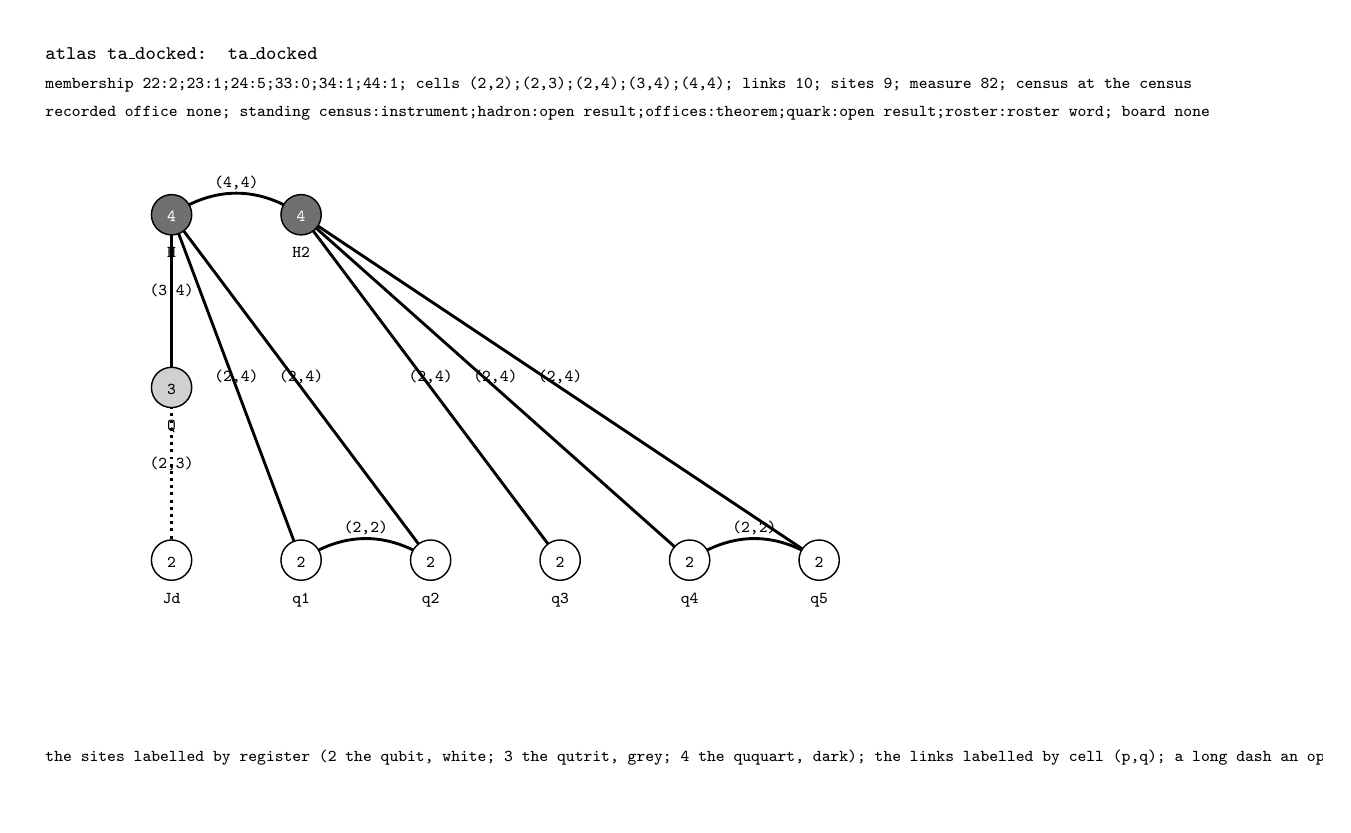
\begin{tikzpicture}[x=0.52pt,y=-0.52pt,baseline]
\clip (0,0) rectangle (900,540);
\fill[white] (0,0) rectangle (900,540);
\node[anchor=base west,inner sep=0pt,text=black,font=\fontsize{6.76}{8.112}\selectfont\ttfamily] at (12,22) {atlas ta\_docked: ta\_docked};
\node[anchor=base west,inner sep=0pt,text=black,font=\fontsize{6.24}{7.488}\selectfont\ttfamily] at (12,42) {membership 22:2;23:1;24:5;33:0;34:1;44:1; cells (2,2);(2,3);(2,4);(3,4);(4,4); links 10; sites 9; measure 82; census at the census};
\node[anchor=base west,inner sep=0pt,text=black,font=\fontsize{5.72}{6.864}\selectfont\ttfamily] at (12,62) {recorded office none; standing census:instrument;hadron:open result;offices:theorem;quark:open result;roster:roster word; board none};
\draw[draw=black,line width=1.04pt] (100,130) .. controls (130,110) and (160,110) .. (190,130);
\node[anchor=base,inner sep=0pt,text=black,font=\fontsize{5.72}{6.864}\selectfont\ttfamily] at (145,111) {(4,4)};
\draw[draw=black,line width=1.04pt] (100,130) -- (100,250);
\node[anchor=base,inner sep=0pt,text=black,font=\fontsize{5.72}{6.864}\selectfont\ttfamily] at (100,186) {(3,4)};
\draw[draw=black,line width=1.04pt] (100,130) -- (190,370);
\node[anchor=base,inner sep=0pt,text=black,font=\fontsize{5.72}{6.864}\selectfont\ttfamily] at (145,246) {(2,4)};
\draw[draw=black,line width=1.04pt] (100,130) -- (280,370);
\node[anchor=base,inner sep=0pt,text=black,font=\fontsize{5.72}{6.864}\selectfont\ttfamily] at (190,246) {(2,4)};
\draw[draw=black,line width=1.04pt] (190,130) -- (370,370);
\node[anchor=base,inner sep=0pt,text=black,font=\fontsize{5.72}{6.864}\selectfont\ttfamily] at (280,246) {(2,4)};
\draw[draw=black,line width=1.04pt] (190,130) -- (460,370);
\node[anchor=base,inner sep=0pt,text=black,font=\fontsize{5.72}{6.864}\selectfont\ttfamily] at (325,246) {(2,4)};
\draw[draw=black,line width=1.04pt] (190,130) -- (550,370);
\node[anchor=base,inner sep=0pt,text=black,font=\fontsize{5.72}{6.864}\selectfont\ttfamily] at (370,246) {(2,4)};
\draw[draw=black,line width=1.04pt,dash pattern=on 1.04pt off 1.56pt] (100,370) -- (100,250);
\node[anchor=base,inner sep=0pt,text=black,font=\fontsize{5.72}{6.864}\selectfont\ttfamily] at (100,306) {(2,3)};
\draw[draw=black,line width=1.04pt] (190,370) .. controls (220,350) and (250,350) .. (280,370);
\node[anchor=base,inner sep=0pt,text=black,font=\fontsize{5.72}{6.864}\selectfont\ttfamily] at (235,351) {(2,2)};
\draw[draw=black,line width=1.04pt] (460,370) .. controls (490,350) and (520,350) .. (550,370);
\node[anchor=base,inner sep=0pt,text=black,font=\fontsize{5.72}{6.864}\selectfont\ttfamily] at (505,351) {(2,2)};
\filldraw[fill={rgb,255:red,112;green,112;blue,112},draw=black,line width=0.52pt] (100,130) circle (14);
\node[anchor=base,inner sep=0pt,text=white,font=\fontsize{6.24}{7.488}\selectfont\ttfamily] at (100,135) {4};
\node[anchor=base,inner sep=0pt,text=black,font=\fontsize{5.72}{6.864}\selectfont\ttfamily] at (100,160) {H};
\filldraw[fill={rgb,255:red,112;green,112;blue,112},draw=black,line width=0.52pt] (190,130) circle (14);
\node[anchor=base,inner sep=0pt,text=white,font=\fontsize{6.24}{7.488}\selectfont\ttfamily] at (190,135) {4};
\node[anchor=base,inner sep=0pt,text=black,font=\fontsize{5.72}{6.864}\selectfont\ttfamily] at (190,160) {H2};
\filldraw[fill=white,draw=black,line width=0.52pt] (100,370) circle (14);
\node[anchor=base,inner sep=0pt,text=black,font=\fontsize{6.24}{7.488}\selectfont\ttfamily] at (100,375) {2};
\node[anchor=base,inner sep=0pt,text=black,font=\fontsize{5.72}{6.864}\selectfont\ttfamily] at (100,400) {Jd};
\filldraw[fill={rgb,255:red,208;green,208;blue,208},draw=black,line width=0.52pt] (100,250) circle (14);
\node[anchor=base,inner sep=0pt,text=black,font=\fontsize{6.24}{7.488}\selectfont\ttfamily] at (100,255) {3};
\node[anchor=base,inner sep=0pt,text=black,font=\fontsize{5.72}{6.864}\selectfont\ttfamily] at (100,280) {Q};
\filldraw[fill=white,draw=black,line width=0.52pt] (190,370) circle (14);
\node[anchor=base,inner sep=0pt,text=black,font=\fontsize{6.24}{7.488}\selectfont\ttfamily] at (190,375) {2};
\node[anchor=base,inner sep=0pt,text=black,font=\fontsize{5.72}{6.864}\selectfont\ttfamily] at (190,400) {q1};
\filldraw[fill=white,draw=black,line width=0.52pt] (280,370) circle (14);
\node[anchor=base,inner sep=0pt,text=black,font=\fontsize{6.24}{7.488}\selectfont\ttfamily] at (280,375) {2};
\node[anchor=base,inner sep=0pt,text=black,font=\fontsize{5.72}{6.864}\selectfont\ttfamily] at (280,400) {q2};
\filldraw[fill=white,draw=black,line width=0.52pt] (370,370) circle (14);
\node[anchor=base,inner sep=0pt,text=black,font=\fontsize{6.24}{7.488}\selectfont\ttfamily] at (370,375) {2};
\node[anchor=base,inner sep=0pt,text=black,font=\fontsize{5.72}{6.864}\selectfont\ttfamily] at (370,400) {q3};
\filldraw[fill=white,draw=black,line width=0.52pt] (460,370) circle (14);
\node[anchor=base,inner sep=0pt,text=black,font=\fontsize{6.24}{7.488}\selectfont\ttfamily] at (460,375) {2};
\node[anchor=base,inner sep=0pt,text=black,font=\fontsize{5.72}{6.864}\selectfont\ttfamily] at (460,400) {q4};
\filldraw[fill=white,draw=black,line width=0.52pt] (550,370) circle (14);
\node[anchor=base,inner sep=0pt,text=black,font=\fontsize{6.24}{7.488}\selectfont\ttfamily] at (550,375) {2};
\node[anchor=base,inner sep=0pt,text=black,font=\fontsize{5.72}{6.864}\selectfont\ttfamily] at (550,400) {q5};
\node[anchor=base west,inner sep=0pt,text=black,font=\fontsize{5.72}{6.864}\selectfont\ttfamily] at (12,510) {the sites labelled by register (2 the qubit, white; 3 the qutrit, grey; 4 the ququart, dark); the links labelled by cell (p,q); a long dash an open dark link of the neutron row; a short dash a docked link at the rule R1};
\end{tikzpicture}
\caption{\texttt{ta\_docked}, beside, hadron row body: 9 sites, 10 links, the measure 82; the links at the cells (2,2), (2,3), (2,4), (3,4), (4,4); the membership 22:2; 23:1; 24:5; 33:0; 34:1; 44:1; 1 docked links at the rule R1 (Q-Jd); at the census of the six cells. Drawn at the anatomy atlas as its web, the sites labeled by register and the links by cell, from the the Higgs and carrier offices at their sinks.}\label{fig:VI-10-D538733-ta-docked-319a00}
\begin{center}\footnotesize\begin{adjustbox}{max width=\linewidth}\begin{tabular}{p{0.26\textwidth}p{0.68\textwidth}}\toprule
recorded office (the slot-count row) & no read of this body at the slot-count row \\
mass register (the mass-register row) & the read htk: the class touching the ququart; the first power 228; the office \texttt{1 437 267 487 777 067/27648000000\textbar{}131/405\textbar{}5069/41472000\textbar{}0}; nonzero; met yes; hubs H; H2; in-legs q-h; dressing 3; ports H2-q3; Q-Jd \\
\bottomrule\end{tabular}\end{adjustbox}\end{center}
\end{figure}
\label{chend:VI-10-D538733-hcos-t1}
\section{The dressing as the Higgs-to-matter leg}\label{mod:VI-10-D539753-w-yklg}
In the Standard Model every charged fermion acquires its mass from its Yukawa coupling to the Higgs field: the mass is the coupling multiplied by the vacuum expectation value over the square root of two, so the Higgs-to-matter vertex of every body is fixed by its mass alone, the leptons and the quarks alike, and the dressing of a body by the Higgs leg is the same mechanism at every generation \cite{Higgs1964,Weinberg1967,Yukawa1935}. The Higgs as the closed hub read is introduced at section~\ref{mod:VI-10-higgs-the-closed-hub-read-its-rows-its-mass-and-its-exponent} and the mass unit with the first power at section~\ref{mod:VIII-1-mass-unit-and-the-first-power}.
The dressing of every body is re-derived as the trace over its (3,4) and (2,4) hub legs under the derived definition of open, the lepton legs at (2,4) and the quark legs at (3,4): the derived definition opens the larger end of every unequal link and washes the far end of every hub leg on the state, so the closed-loop act closes at every hub leg and the trace is the far-end dimension, 2 at a (2,4) leg and 3 at a (3,4) leg; the leg trace at the five bodies, 8, 64, 512, 27 and 81, agrees with the established dressings 1, 9, 27, 9 and 27 at none of the five.
The hub is the larger end at every (2,4) and (3,4) leg, the letters agreeing with the ends table of the larger-end definition at the three bodies it carries, 490 of 490, and the traces are reproduced at 5 of 5. The first body at which the leg trace parts from the dressing is the electron, the trace 8 over its three (2,4) legs against the established value 1, named with both values; the parting stands at the three (2,4) legs of the electron and at the entering (3,4) leg of each nucleon, the legs the established values pass. The (3,4) legs alone give 3, 9, 27, 27 and 81, agreeing at the muon and the tau alone, and the standing definition, which opens the smaller end and passes every hub leg, gives 1 at every body, agreeing at the electron alone.
The result is an open result: the leg trace under the derived definition parts from the established dressing at the first body, the electron, and at the nucleons; no comparison with observation is made here.
What stays open is a result reproducing the dressing law 3 to the k at the five bodies at the first face, found at none; the closed-leg dressing at the hub legs alone (section~\ref{mod:VIII-1-D539465-w-lhlc}) stands beside at its own body parting.
\section{The Higgs quartic as the ratio of offices}\label{mod:VI-10-D540200-hqrt-t1}
\begin{chtheorem}[The Higgs quartic as the ratio of offices]\label{box:VI-10-D540200-hqrt-t1:1}
The Higgs quartic is the ratio of two offices at every Higgs-form sink: the same ratio the quartic results spell, a Higgs face over a vacuum face squared, is an exact element of the field of root two and root three at the office of every one of the 10123 Higgs-form sinks of the fourth column over the vacuum office 6561 of that column squared, 60738 of 60738 at the six readings, equal to the quartic spelling of the column at 10123 of 10123 at the first and the fourth reading; at the Higgs word of the fixed library the quartic is the hub-face office over 6561 squared and the leg-face office over 256 squared, equal to the quartic cells of the Higgs-and-carrier-offices result and the quartic of the column; the vacuum office is located at six of six readings, equal to the Higgs-and-carrier, vacuum-expectation and Higgs-attachment cells; a theorem of the one rule at the Higgs-form sinks under the axiom text, stated without comparison with observation.
The first face, the same ratio at the Higgs-form sink office over the vacuum office squared of the fourth column an exact cell, reads yes, the sinks defined at 10123 of 10123 with the word face re-met, the vacuum office located at six of six and the ratios exact at 60762 of 60762; the second face, no Higgs-form sink or no vacuum office at the column named, reads no, the first undefined sink none, the first unread ratio none, the first parting none.
\end{chtheorem}
\chstanding{a theorem}
\chdeps{Definitions 1.1 to 1.6 and Theorems 200.1 to 200.3 and Open result 200.4}{no theorem beyond it at this release}
The quartic coupling of the Higgs is spelled at the foregoing results as a Higgs face over a vacuum face squared, and the question is whether that spelling is one exact cell when the Higgs face is read as the office of a Higgs-form sink by the one rule and the vacuum face as the vacuum office of the saturation census at its fourth column. It is, at every one of the 10123 Higgs-form sinks of that column and at every one of the six readings of the vacuum office, the registers 6561, 81, 65536, 256, 16 and 256, so that 60738 ratios are exact elements of the field whose product with the vacuum office squared returns the office they came from; the Higgs word of the fixed library gives the same ratio at its hub face and at its leg face, equal to the cells of the foregoing results. The quartic is a ratio of two offices and needs no observed value and no unit.
\begin{chbridge}
The quartic coupling of the Higgs field is the coefficient of the fourth power of the field in the scalar potential of the Standard Model, fixed in the standard account by the Higgs mass and the vacuum expectation value through the relation that the mass squared is twice the quartic multiplied by the vacuum expectation value squared \cite{Weinberg1967,Peskin1995}. The correspondence is by name.
\end{chbridge}
\begin{chproof}[exhaustive census with its exact part]
The premises of this derivation are the axiom and the six definitions of chapter~\ref{mod:FRAMEWORK}, the Higgs as the closed hub read of chapter~\ref{mod:VI-10-higgs-the-closed-hub-read-its-rows-its-mass-and-its-exponent}, a theorem, the body-alone office rule of chapter~\ref{mod:VIII-2-body-alone-office-rule}, a theorem, the Higgs and carrier offices at their sinks of the present chapter, a theorem, and the vacuum register of the chapter titled The electroweak table (chapter~\ref{mod:VI-9-electroweak-table}, among the instruments), an instrument. The chain of premises runs back to the axiom through those chapters, and the longest such chain in this compendium is twelve chapters long.
\textit{The exact part.} The Higgs word of the fixed library carries at its hub face the office $\tfrac{46656001681}{182250000}$ and the vacuum office at the first reading is the register of the clauses, the (3,3) register of the common support 81 to the order exponent two, $6561$, so the quartic at the hub face is
\begin{equation} \lambda_{\mathrm{hub}} = \frac{46656001681}{182250000\cdot 6561^{2}} = \frac{46656001681}{182250000\cdot 43046721}, \end{equation}
an exact rational, equal to the quartic cell of the Higgs-and-carrier-offices result; at the leg face the quartic is the leg-face office over the port register $256$ squared, an exact element with a root-three coordinate, equal to the leg-face cell alike. The six readings of the vacuum office are $6561$, $81$, $65536$, $256$, $16$ and $256$, each equal to the vacuum register of the Higgs-and-carrier-offices result at the same reading. The figure draws the Higgs word with its attachment and its leg.
\textit{The census.} By exhaustive enumeration of the 10123 Higgs-form sinks of the fourth column of the saturation census, 665 within its material at the types charged 158, neutral 487 and dark 20 and 9458 beyond it, by hub count 8, 92, 878, 716, 1676, 654, 4917, 108 and 1074 at the hubs two to ten: the property tested at each sink is that its office by the one rule is an exact nonzero element of the field with a positive closure, and that its ratio over the vacuum office squared at each of the six readings is an exact element returning the office when multiplied back; the counts by class are the offices defined at 10123 of 10123 with the closure positive at 10123 of 10123, the ratios exact at 60738 of 60738 at the sinks and 24 of 24 at the faces, the products returning the office at 60756 of 60756, and the column spelling re-met at 10123 of 10123 at the first and at the fourth reading. The smallest case worked is the Higgs word above; the first sink within the material and the first beyond are recorded with their four coordinates.
\textit{The check.} The counter-tests alter the construction singly and read what moves. Striking the vacuum office at every reading moves forty-seven cells and the second face names no vacuum office. Striking the Higgs-form sinks moves twenty-one cells and the second face names no sink. Striking the square, the vacuum office at the first power, moves thirty-five cells with every re-meet parting. Striking the ninth-text passage unmeets the gate. Striking the closure at the first sink moves eight cells. Each alteration moves the cells it names. The result was reproduced by an independent route, two engines built apart, the exact-fraction route against the second route, equal at every cell, with the sixteen controls the same.
\chcert{10123}
\begin{figure}[h]\centering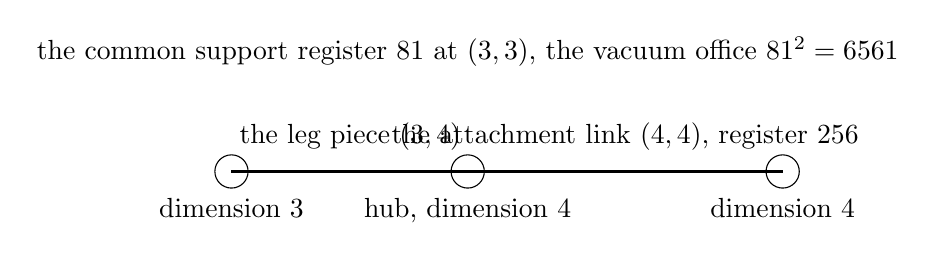
\begin{tikzpicture}[scale=1]
\filldraw[fill=white] (0,0) circle (6pt) node[below=6pt] {hub, dimension 4};
\filldraw[fill=white] (4,0) circle (6pt) node[below=6pt] {dimension 4};
\filldraw[fill=white] (-3,0) circle (6pt) node[below=6pt] {dimension 3};
\draw[thick] (0,0) -- (4,0); \draw[thick] (-3,0) -- (0,0);
\node at (2,0) [above=4pt] {the attachment link $(4,4)$, register $256$};
\node at (-1,0) [above=4pt, xshift=-14pt] {the leg piece $(3,4)$};
\node at (0,1) [above=6pt] {the common support register $81$ at $(3,3)$, the vacuum office $81^{2} = 6561$};
\end{tikzpicture}\caption{The Higgs word at its hub: the attachment link of genre (4,4) and the leg piece of genre (3,4), with the registers that spell the vacuum office at its first and fourth readings.}\end{figure}
\end{chproof}
\par\medskip\noindent{\itshape The Higgs read, Part XII turns to the processes in which mass is released.}\label{narr:close:6-10}\par
